%%%%%%%%%%%%%%%%%%%%%%%%%%%%%%%%%%%%%%%%%
% Beamer Presentation
% LaTeX Template
% Version 1.0 (10/11/12)
%
% This template has been downloaded from:
% http://www.LaTeXTemplates.com
%
% License:
% CC BY-NC-SA 3.0 (http://creativecommons.org/licenses/by-nc-sa/3.0/)
%
%%%%%%%%%%%%%%%%%%%%%%%%%%%%%%%%%%%%%%%%%

%----------------------------------------------------------------------------------------
%	PACKAGES AND THEMES
%----------------------------------------------------------------------------------------

\documentclass[xcolor=table,usenames,dvipsnames]{beamer}

\mode<presentation> {

% The Beamer class comes with a number of default slide themes
% which change the colors and layouts of slides. Below this is a list
% of all the themes, uncomment each in turn to see what they look like.

%\usetheme{default}
%\usetheme{AnnArbor}
%\usetheme{Antibes}
%\usetheme{Bergen}
%\usetheme{Berkeley}
%\usetheme{Berlin}
%\usetheme{Boadilla}
%\usetheme{CambridgeUS}
%\usetheme{Copenhagen}
%\usetheme{Darmstadt}
%\usetheme{Dresden}
%\usetheme{Frankfurt}
%\usetheme{Goettingen}
%\usetheme{Hannover}
%\usetheme{Ilmenau}
%\usetheme{JuanLesPins}
%\usetheme{Luebeck}
\usetheme{Madrid}
%\usetheme{Malmoe}
%\usetheme{Marburg}
%\usetheme{Montpellier}
%\usetheme{PaloAlto}
%\usetheme{Pittsburgh}
%\usetheme{Rochester}
%\usetheme{Singapore}
%\usetheme{Szeged}
%\usetheme{Warsaw}

% As well as themes, the Beamer class has a number of color themes
% for any slide theme. Uncomment each of these in turn to see how it
% changes the colors of your current slide theme.

%\usecolortheme{albatross}
%\usecolortheme{beaver}
%\usecolortheme{beetle}
%\usecolortheme{crane}
%\usecolortheme{dolphin}
%\usecolortheme{dove}
%\usecolortheme{fly}
%\usecolortheme{lily}
%\usecolortheme{orchid}
%\usecolortheme{rose}
%\usecolortheme{seagull}
%\usecolortheme{seahorse}
%\usecolortheme{whale}
%\usecolortheme{wolverine}

%\setbeamertemplate{footline} % To remove the footer line in all slides uncomment this line
%\setbeamertemplate{footline}[page number] % To replace the footer line in all slides with a simple slide count uncomment this line

%\setbeamertemplate{navigation symbols}{} % To remove the navigation symbols from the bottom of all slides uncomment this line
}

\usepackage{graphicx} % Allows including images
\usepackage{booktabs} % Allows the use of \toprule, \midrule and \bottomrule in tables
\usepackage{tikz}
\usepackage{verbatim}
\usepackage{pgfplots}
\usepackage{listings}
\newcommand{\dd}{\partial}
%----------------------------------------------------------------------------------------
%	TITLE PAGE
%----------------------------------------------------------------------------------------

\usepackage[utf8]{inputenc}
\usepackage[russian]{babel}
\usepackage{environ}
\title[АСДЦвТОЧ]{Алгоритмы сопровождения динамических целей в трехмерных облаках точек} % The short title appears at the bottom of every slide, the full title is only on the title page
\tikzset{every picture/.style={/utils/exec={\sffamily}}}
\date{\today} % Date, can be changed to a custom date
\author{Щелчков Дмитрий}
\setbeamercovered{invisible}
\setbeamercovered{%
  again covered={\opaqueness<1->{15}}}
%\usepackage[T2A]{fontenc}

%\usepackage{fontspec}
%\setsansfont{xkcd}
\usepackage{xifthen}



%  \addtobeamertemplate{frametitle}{
%   \let\insertframetitle\insertsectionhead}{}
%\makeatletter
%  \CheckCommand*\beamer@checkframetitle{\@ifnextchar\bgroup\beamer@inlineframetitle{}}
%  \renewcommand*\beamer@checkframetitle{\global\let\beamer@frametitle\relax\@ifnextchar\bgroup\beamer@inlineframetitle{}}
%\makeatother
%\addtolength{\jot}{1em}
\begin{document}

\begin{frame}
\titlepage % Print the title page as the first slide
\end{frame}

\begin{frame}
\frametitle{Overview} % Table of contents slide, comment this block out to remove it
\tableofcontents % Throughout your presentation, if you choose to use \section{} and \subsection{} commands, these will automatically be printed on this slide as an overview of your presentation
\end{frame}
 % Лидар, KITTI, MOTA, скорее всего будут в презентации Антона
 % Основная идея - построить реалтаймовый трекер на лидарных данных
\begin{frame}
\frametitle{LIDAR}
\begin{columns}
\begin{column}{0.5\textwidth}
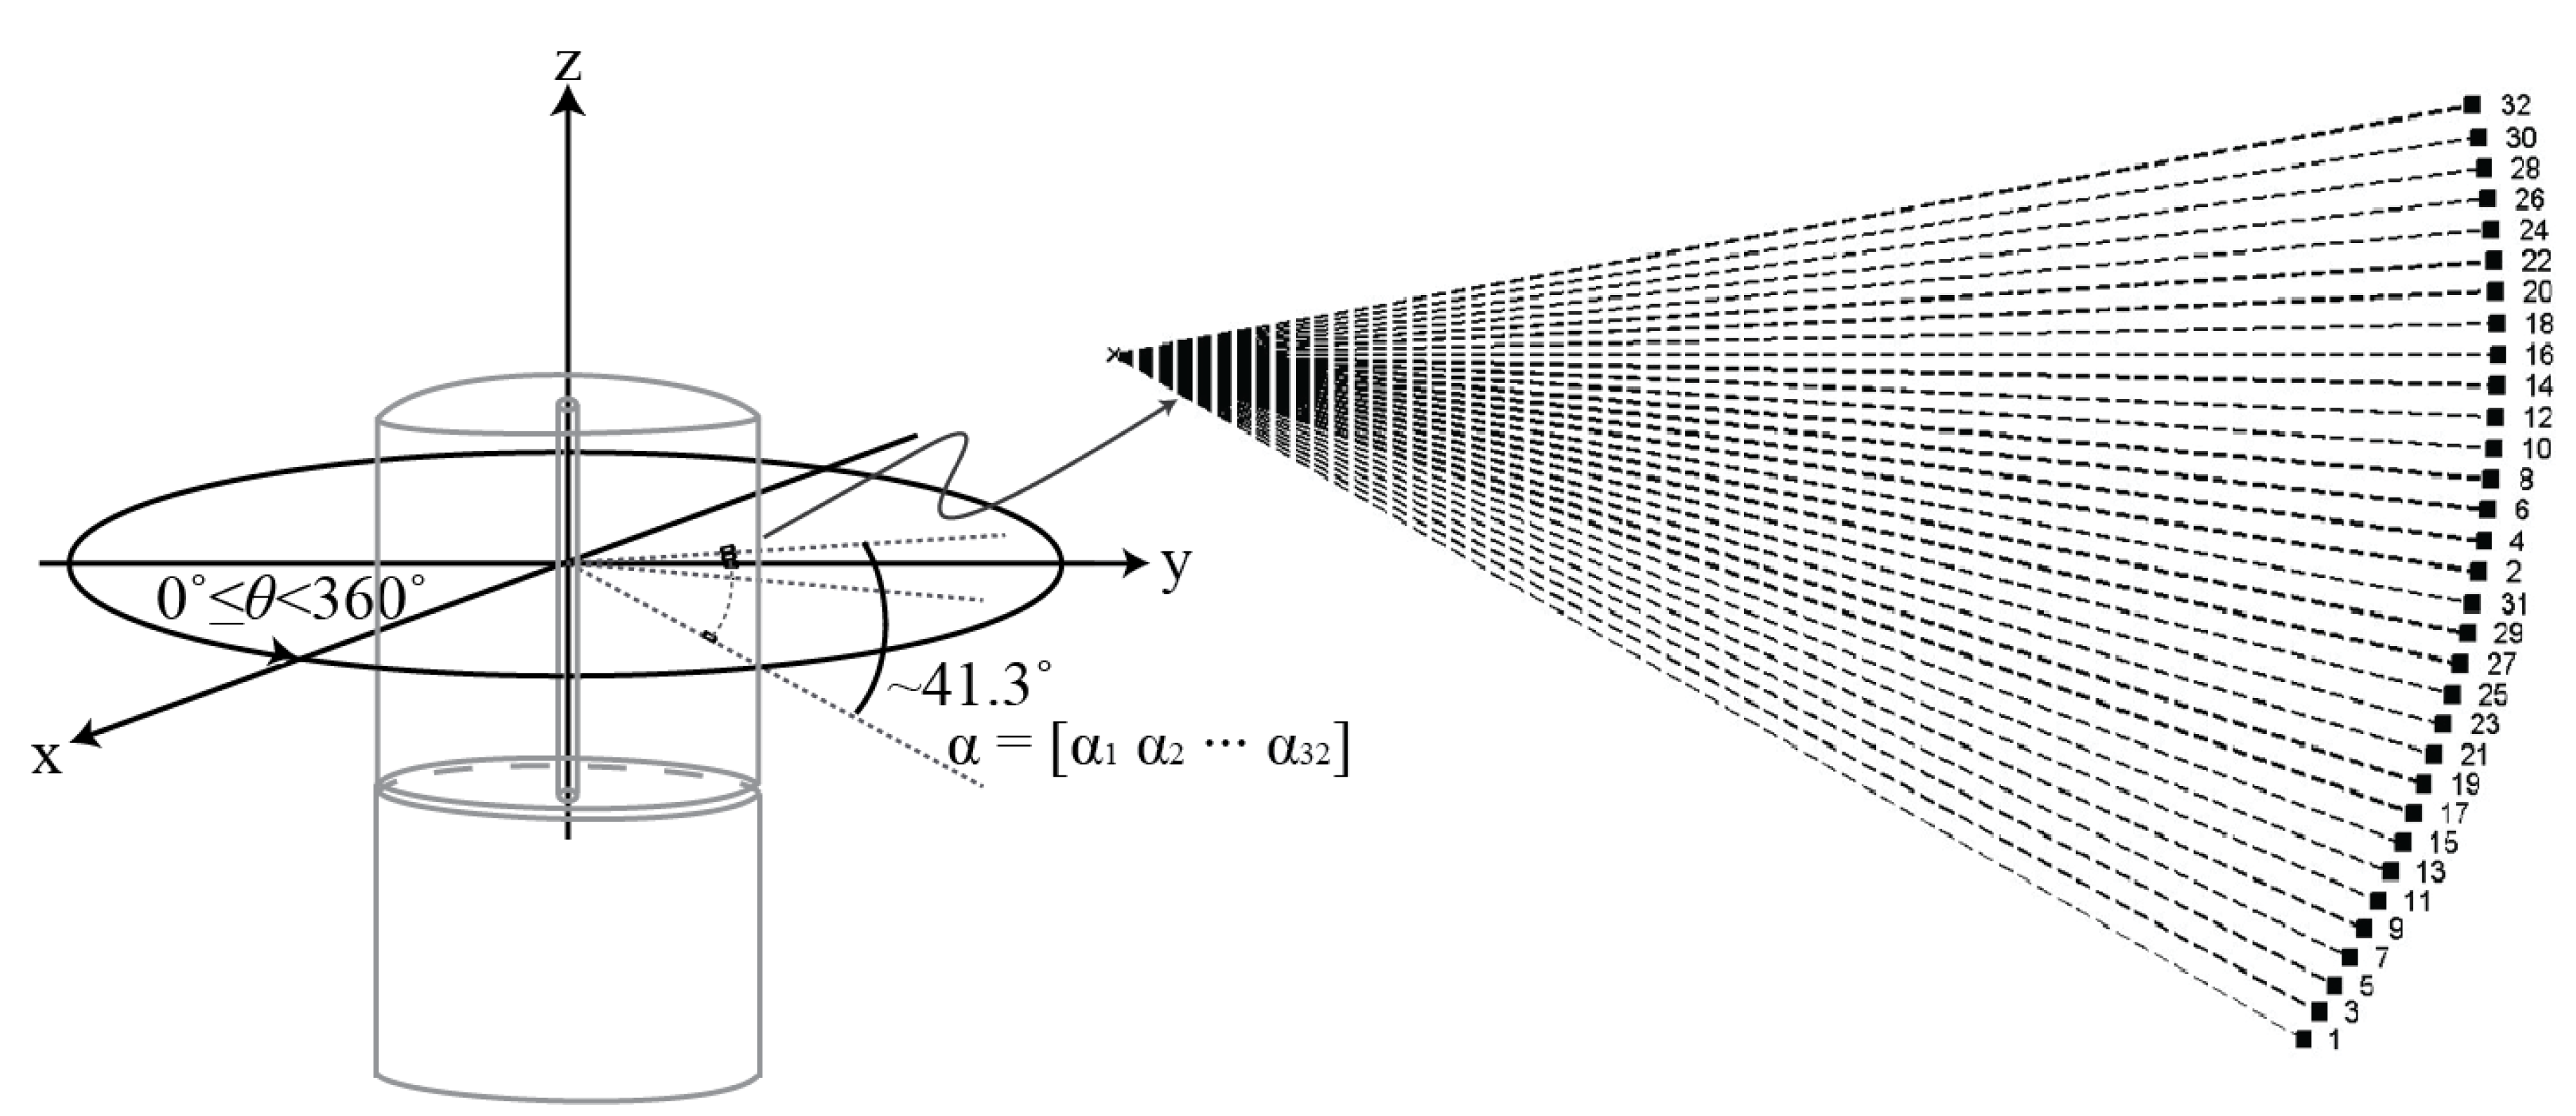
\includegraphics[width=\textwidth, height=0.5\textheight]{img/lidar.png}
\end{column}
\begin{column}{0.5\textwidth}
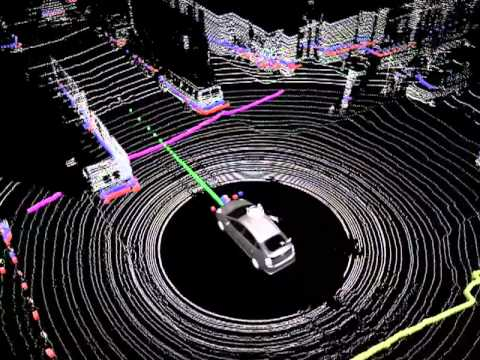
\includegraphics[width=\textwidth, height=0.5\textheight]{img/lidar_data.jpg}
\end{column}
\end{columns}
\begin{itemize}
\item 64 beams
\item 10 Hz
\end{itemize}
\end{frame}
\begin{frame}
\frametitle{KITTI}
\begin{columns}
\begin{column}{0.7\textwidth}
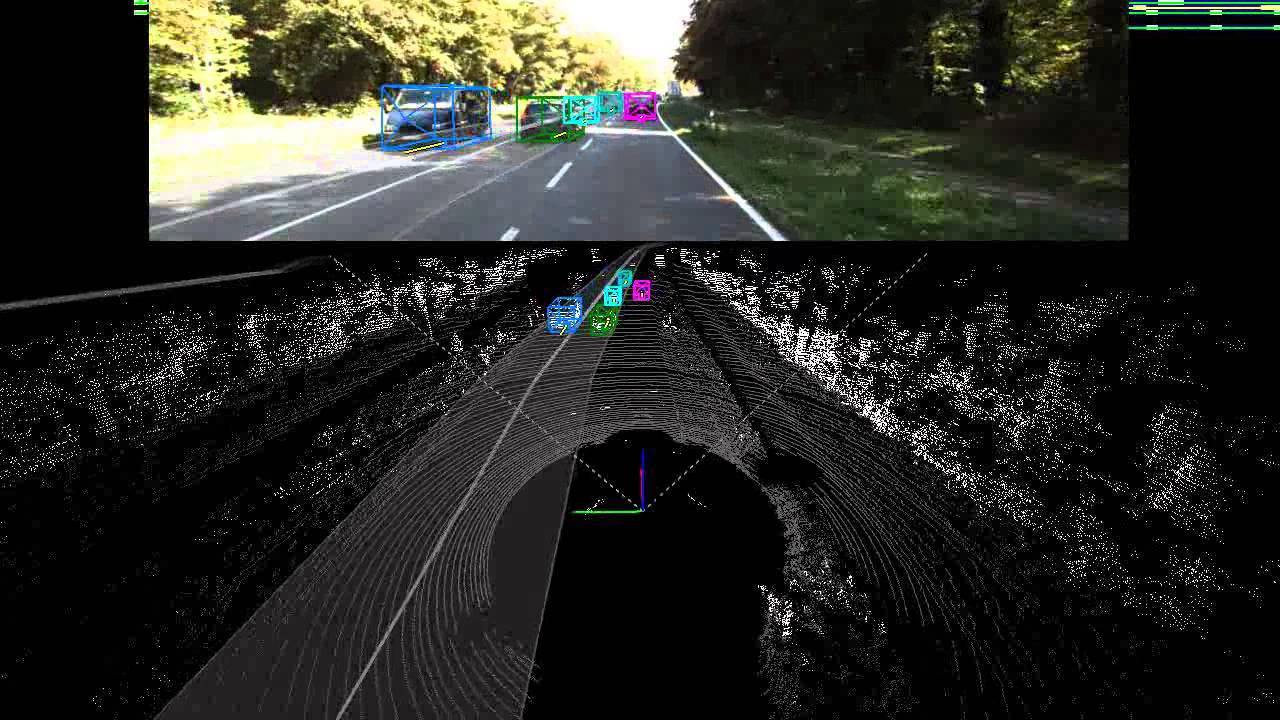
\includegraphics[width=\textwidth, height=0.7\textheight]{img/KITTI_sample.jpg}
\end{column}
\begin{column}{0.3\textwidth}
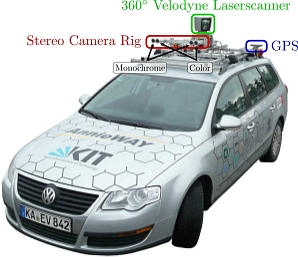
\includegraphics[width=\textwidth]{img/KITTI_car.jpg}
\end{column}
\end{columns}
\begin{itemize}
\item 50 tracklets from 10 to 45 seconds each
\item Bbox for each object
\end{itemize}
\end{frame}
%добавить ниже метрики
\begin{frame}
\frametitle{Задача сегментации}
\begin{center}
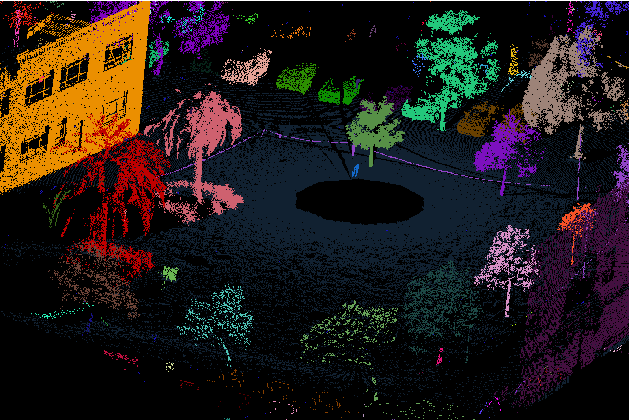
\includegraphics[height=0.7\textheight]{img/segmentation.png}
\end{center}
\begin{itemize}
\item Cars and people are the only important segments
\end{itemize}
\end{frame}
\begin{frame}
\frametitle{Задача детекции и трекинга}
\begin{center}
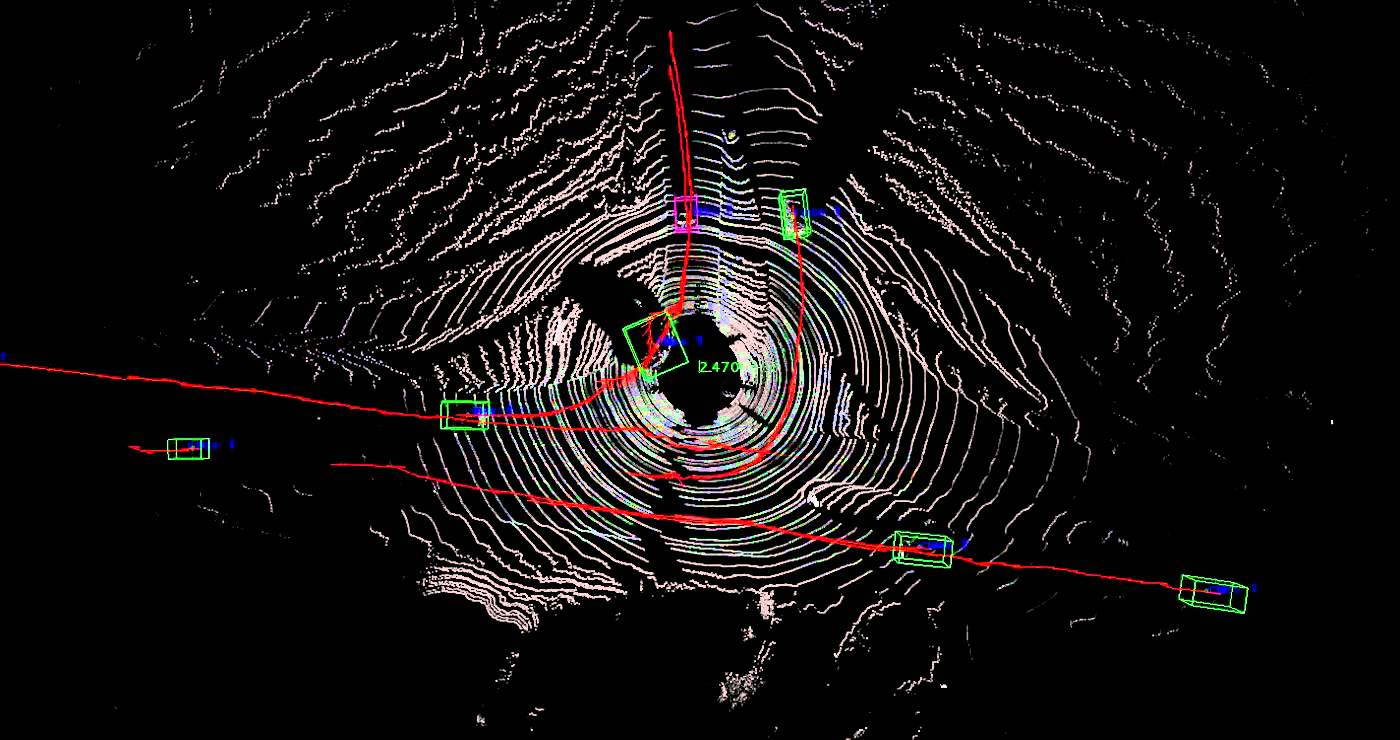
\includegraphics[width=0.9\textwidth]{img/tracking.jpg}
\end{center}
\begin{itemize}
\item Problems: occlusion, mismatch between frames
\item One may be or may not be interested in direction, acceleration and speed
\end{itemize}
\end{frame}
\begin{frame}
Корреляционные фильтры - пример из картинок, хочется кернел денсити овер юнион
\end{frame}
\begin{frame}
\frametitle{Robot Operating System (ROS)}
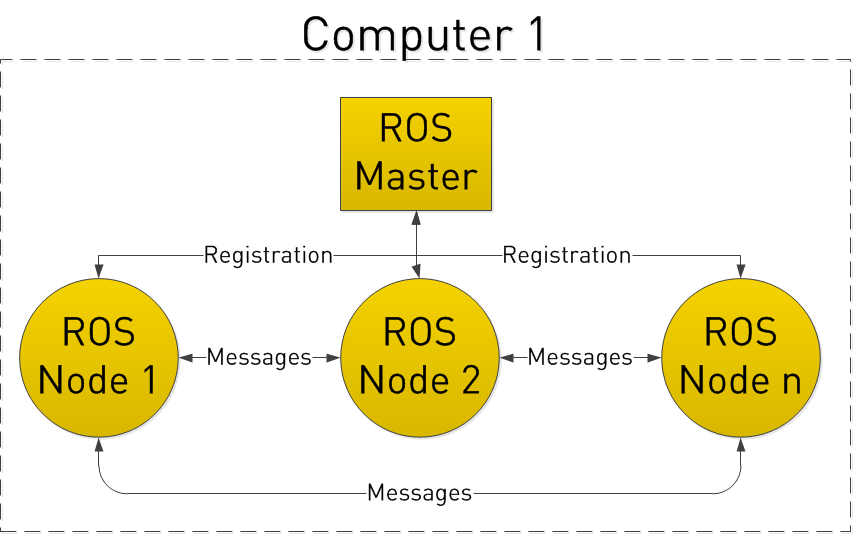
\includegraphics[height = 0.7\textheight]{img/ros.png}
\begin{flushright}
\end{flushright}
\end{frame}
\begin{frame}
\frametitle{Robot Operating System (ROS): tracker graph}
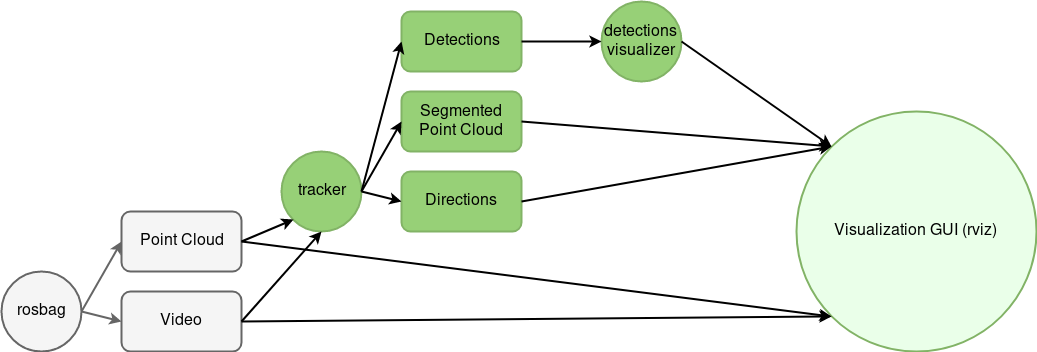
\includegraphics[width = \textwidth]{img/ros_graph.png}
\end{frame}
\begin{frame}
\frametitle{Pipeline}
\begin{enumerate}
\item Segmentation
\item Association
\item Tracking
\end{enumerate}
\end{frame}
\begin{frame}
\frametitle{Segmentation}
\begin{columns}
\begin{column}{0.5\textwidth}
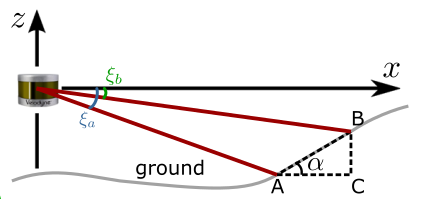
\includegraphics[width=\textwidth]{img/ground_alpha.png}
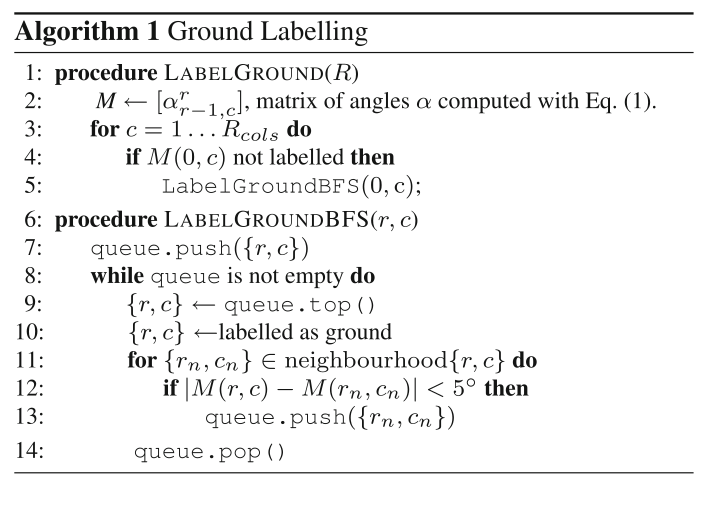
\includegraphics[width=\textwidth]{img/ground_algo.png}
\end{column}
\begin{column}{0.5\textwidth}
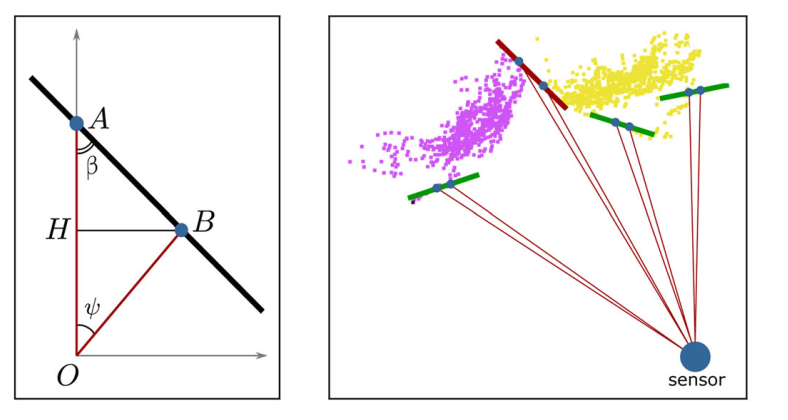
\includegraphics[width=0.9\textwidth]{img/alpha.png}
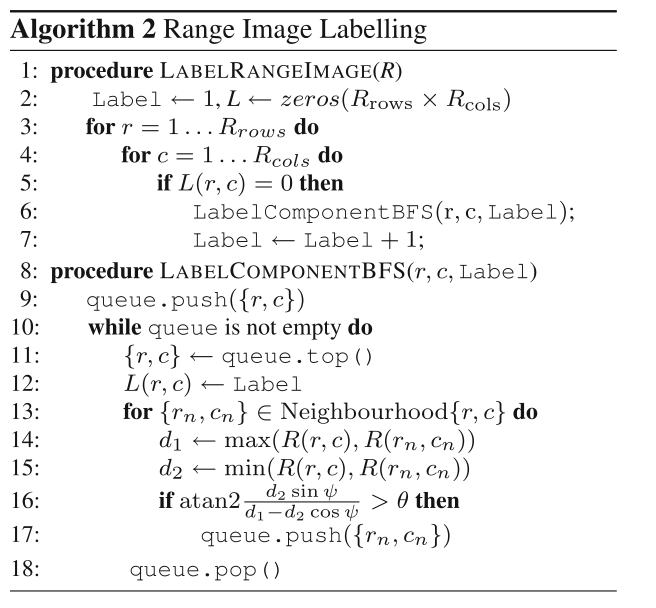
\includegraphics[width=0.9\textwidth]{img/segmentation_algo.png}
\end{column}
\end{columns}
\end{frame}
\begin{frame}
\frametitle{Segmentation: troubleshooting}
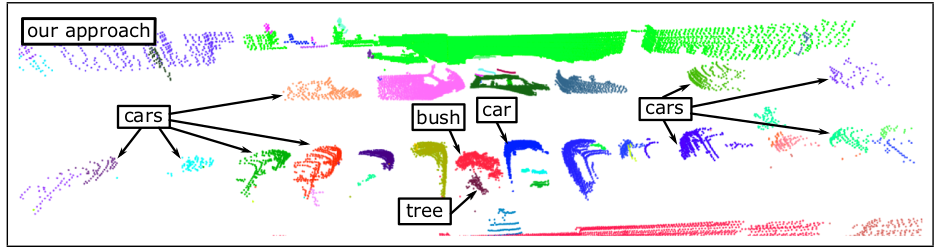
\includegraphics[width=0.9\textwidth]{img/segmentation_sample.png}
We need only good segmentation of moving objects
\begin{columns}
\begin{column}{0.5\textwidth}
There's a number of problems:
\begin{enumerate}
\item Undersegmentation of the ground
\item Incapability to work in the presence of plants
\end{enumerate}
\end{column}
\begin{column}{0.5\textwidth}
\begin{enumerate}
\item Normal based approach
\item Trees and grass removal algorithm
\end{enumerate}
\end{column}
\end{columns}
\end{frame}
\begin{frame}
\frametitle{Segmentation: trees}
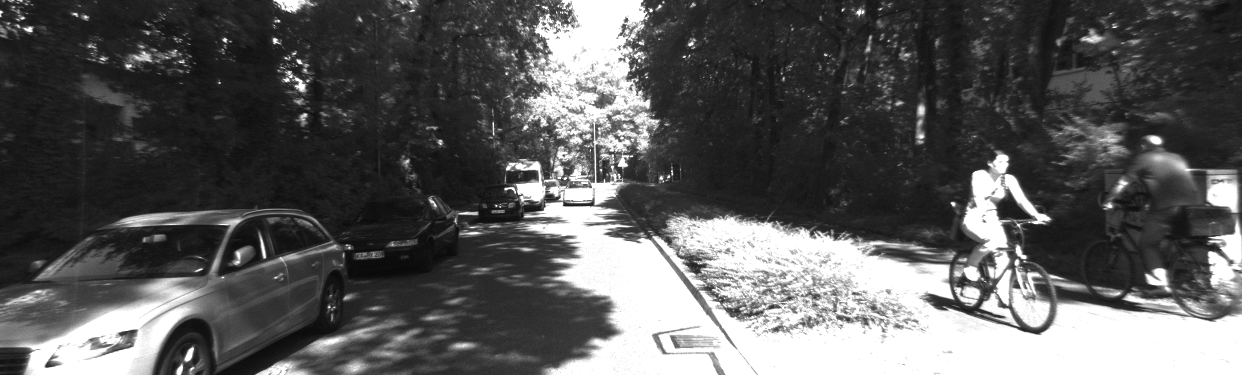
\includegraphics[width = 0.95\textwidth]{img/trees_picture.png}
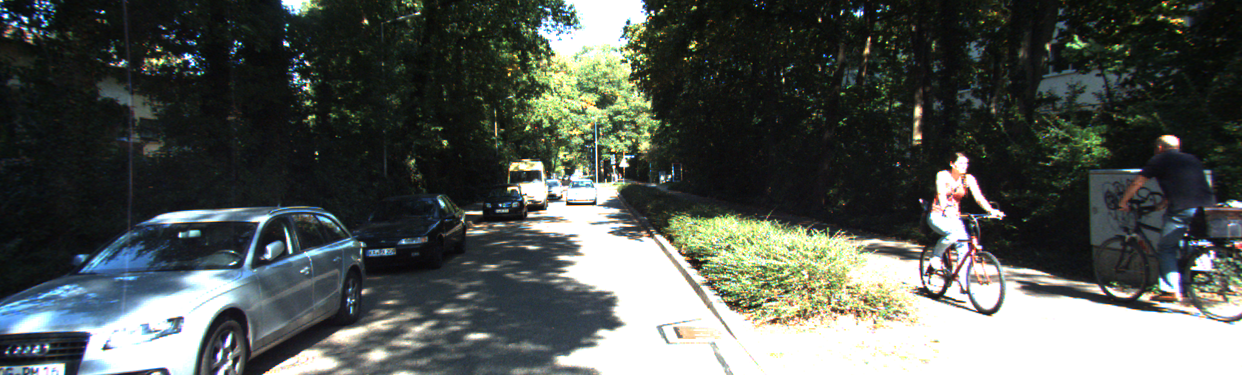
\includegraphics[width = 0.95\textwidth]{img/coloured_trees_picture.png}
\end{frame}
\begin{frame}
\frametitle{Segmentation: trees removal}
\begin{columns}
\begin{column}{0.4\textwidth}
\begin{itemize}
\item Create local approximation of an object shape
\item Check deviation of a point
\item Remove points with many outliers in neighbourhood
\end{itemize}
\end{column}
\begin{column}{0.6\textwidth}
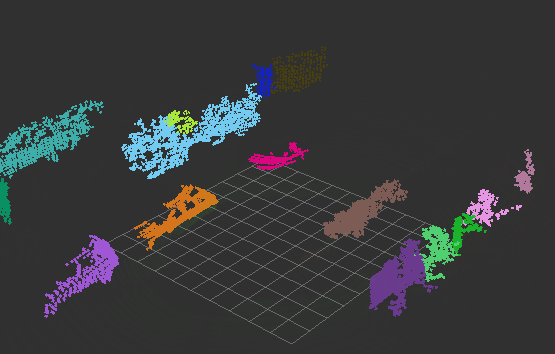
\includegraphics[height=0.4\textheight]{img/before_plants_removal.png}
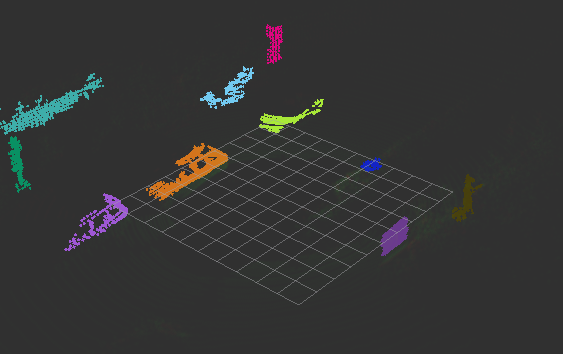
\includegraphics[height=0.4\textheight]{img/plants_removal.png}
\end{column}
\end{columns}
Runtime < 50ms
\end{frame}

\begin{frame}
\frametitle{Segmentation: notes}
\begin{itemize}
\item Not moving obstacles doesn't matter
\item Only cars and pedestrians segmentation necessary
\item Car shapes should be accurate
\end{itemize}
\end{frame}
\begin{frame}
Трекинг - ICP + kernel correlation filter + kalman filter as baseline
Нет данных чтобы обучить корреляционный фильтр (
\end{frame}
\begin{frame}
Корреляционный фильтр на PointNet
\end{frame}
\end{document}
